%!TEX root = ../dokumentation.tex

\chapter{Der Minimax-Algorithmus}
In diesem Kapitel wird erläutert, wie die bestehende Implementierung der Schach-KI aufgebaut ist und wie diese funktioniert. Die vorgestellten Implementierungen können ebenfalls auf \textit{GitHub} unter \url{https://github.com/felixwortmann/chess} abgerufen werden.

\section{Das Schach-Spiel}
Zunächst werden die Grundlagen des Schach-Spiels erläutert. Es handelt sich bei Schach um ein Brettspiel für zwei Spieler, wobei einer der Spieler mit der Farbe Weiß, der andere mit der Farbe Schwarz spielt. Jeder der Spieler hat jeweils 16 Figuren, davon acht Bauern, jeweils zwei Springer, Läufer und Türme, eine Dame sowie einen König. Der Spieler der weißen Farbe beginnt stets, wobei jeder Spieler die folgenden Züge mit den jeweiligen Figuren ausführen kann:

\begin{itemize}
    \item Bauer -- Die schwächste Figur im Spiel, kann pro Zug ein Feld nach vorne rücken (falls es der erste Zug des Bauern ist, kann dieser ein oder zwei Felder vorrücken) und gegnerische Figuren schlagen, falls sie diagonal ein Feld vor ihm liegen
    \item Springer -- Die einzige Figur im Spiel, die über andere Figuren "`springen"' kann. Das Zugmuster des Springers gleicht einem L, da er zwei Felder in eine Richtung, dann ein Feld orthogonal zur Seite ziehen kann. Die Figuren, die er überspringt, werden nicht beeinflusst
    \item Läufer -- Der Läufer kann sich auf einer Diagonale in alle Richtungen bewegen
    \item Turm -- Türme können sich ähnlich den Läufern auf einer Linie bewegen, jedoch nicht diagonal sondern horizontal und vertikal
    \item Dame -- Die Dame hat die meisten Möglichkeite zum Zug: diagonal, horizontal, vertikal sowie alle umliegenden Felder
    \item König -- Der König kann sich zwar nur pro Zug ein Feld in eine beliebige Richtung bewegen, ist aber insofern die wichtigste Figur des Spiels, als dass er über Niederlage eines Spieler unterscheiden kann: Steht eine gegnerische Figur so, dass sie im nächsten Zug den König schlagen könnte, ist er \textit{schach} gesetzt; hat der Spieler zusätzlich keine Mögichkeit, den König zu schützen (durch Zug des Königs auf ein anderes Feld, Blockieren der Angriffslinie durch eine andere Figur oder schlagen der bedrohenden Figur), spricht man von \textit{Schachmatt} und der gegnerische Spieler hat gewonnen
\end{itemize}

Eine Möglichkeit, wie das Spiel enden kann, wurde bereits erwähnt: das \textit{Schachmatt}. Bei Schach handelt es sich um ein sogenanntes \textit{Nullsummenspiel}, sodass, analog zu Spielen wie beispielsweise \textit{Tic Tac Toe} oder \textit{Vier gewinnt}, das Spiel nur auf drei Weisen enden kann: Spieler A (weiß) gewinnt, Spieler B (schwarz) gewinnt oder es herrscht Gleichstand, \textit{Remis} genannt.

Die drei Möglichen stellen sich folgendermaßen dar:

\begin{enumerate}
    \item Weiß gewinnt: Schwarz wurde schachmatt gesetzt oder hat aufgegeben
    \item Schwarz gewinnt: Weiß wurde schachmatt gesetzt oder hat aufgegeben
    \item Remis: Spieler einigen sich auf ein Remis, einer der Spieler steht \textit{patt} (keine möglichen Züge, der König ist jedoch nicht schachmatt gesetzt), beide Spieler haben nicht genug Figuren, um das Spiel zu gewinnen oder, die letzte Variante, eine bestimmte Anzahl an Zügen wurde (wiederholt) ausgeführt
\end{enumerate}

\section{Grundgedanke einer Schach-KI}
Der grundlegende Ansatz einer Schach-KI besteht darin, dass das Programm alle möglichen Züge analysiert und den besten Zug auswählt. Aufgrund der oben erwähnten Anzahl an möglichen Zügen für jeden Spieler, wächst die Zahl der möglichen Spiele, die daraus resultieren, jedoch stark an. Es wäre daher de facto unmöglich, \textit{alle} Züge einer kompletten Schach-Partie zu analysieren, da kein Computer der Welt je genug Speicherplatz haben würde, um alle möglichen Ergebnisse abzuspeichern: Die Anwendung der Rechnung von \textit{Claude Shannon} ergibt eine geschätzte Untergrenze von $10^{120}$ möglichen Spielpositionen in einer gesamten Schachpartie\footcite{shannon}; die Anzahl der Atome im beobachtbaren Universum beträgt jedoch schätzungsweise $10^{80}$\footcite{merz}. Somit wird es, unabhängig von der Rechenleistung, nie möglich sein, alle unterschiedlichen Spiel-Ausgänge abzuspeichern.

Entscheidet man sich nun, statt aller möglichen Züge, nur bis zu einer bestimmten Tiefe zu suchen, verringert sich die Anzahl an möglichen Zügen zwar, bleibt aber dennoch zu hoch, da sich die Anzahl an möglichen Spiel-Zuständen mit jedem vollen Zug um den Faktor $10^{3}$ erhöht\footcite{shannon}. Es benötigt also einen Algorithmus, welcher effizient durch eine begrenzte Anzahl möglicher Züge geht und analysiert, welcher dieser Züge die beste Folgeposition zur Folge hat. Der genutzte Algorithmus ist der \textit{Minimax-Algorithmus}, genauer die Variante \textit{Negamax}, welche jedoch de facto analog zu dem Standard-Minimax-Algorithmus funktioniert und lediglich die Rückgabewerte so anpasst, dass beide Spieler maximierend sind, statt der Standadvariante in der der Spieler der Farbe Weiß maximierend und der Spieler der Farbe Schwarz minimierend ist -- dies ist auch der Grund für die Namensgebung des Algorithmus.

\section{Funktionsweise des Minimax-Algorithmus}
Der Minimax-Algorithmus funktioniert \textit{rekursiv}, das heißt, dass die Funktion sich selbst so lange aufruft, bis die Abbruchbedingung erreicht wird. Die Abbruchbedingungen in diesem Kontext sind, dass entweder 

\begin{enumerate}
    \item die maximale Suchtiefe erreicht wird oder
    \item keine weiteren Züge zur Analyse vorhanden sind.
\end{enumerate}

Abbildung~\ref{fig:minimax} stellt den Ablauf des Algorithmus dar. Zu sehen ist ein \textit{Baum}, welcher die verschiedenen Zustände durch Zahlen abbildet. Diese Zahlen können sowohl negativ als auch positiv sein; die negativen Zahlen sind dabei gut für den minimierenden Spieler (Schwarz), während positive Zahlen gut für den maximierenden Spieler (Weiß) sind. Außerdem sind die Werte $+\infty$ und $-\infty$ zu sehen -- diese Werte stellen eine Schachmatt-Position dar, können jedoch auch anders implementiert werden. Der Algorithmus geht so vor, dass er rekursiv durch den abgebildeten Baum iteriert und den Pfad raussucht, welcher zum besten Ergebnis (in der Abbildung wäre dies der Pfad, der zu $+\infty$ führt) führt.

\begin{figure}[H]
	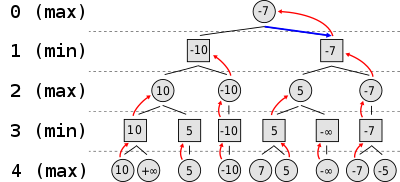
\includegraphics[width=.90\textwidth]{minimax.svg.png}
	\caption{Überblick über die Vorgehensweise des Minimax-Algorithmus\footnotemark}
	\label{fig:minimax}
\end{figure}
\footnotetext{\cite{minimax}}

Die Werte werden mithilfe einer weiteren Funktion berechnet, indem verschiedene Faktoren in die Berechnung miteinbezogen werden. Beispiele für solche Faktoren sind:

\begin{itemize}
    \item Die Anzahl der jeweiligen Figuren, die verschiedenen Figurtypen haben dabei verschiedene Werte: Eine Dame entspricht dabei beispielsweise dem Wert von neun Bauern
    \item Die Position der einzelnen Figuren. Ein Springer im Zentrum ist wertvoller als ein Springer am Rand, da er im Zentrum mehr Zugmöglichkeiten hat
    \item Die Tatsache, ob ein Schachmatt herrscht
\end{itemize}

Die Verwendung des Minimax-Algorithmus allein wird zwar eine intelligente Berechnung der Züge erlauben, jedoch, aufgrund der weiterhin großen Anzahl an möglichen Zügen, keine hohe Suchtiefe ermöglichen. Um die Berechnungsdauer zu verringern -- und somit eine hohere Suchtiefe zu ermöglichen -- bestehen daher Verbesserungsmöglichkeiten. Die implementierten Verbesserungen sind dabei das sogenannte \textit{Alpha-Beta-Pruning}, die Verwendung einer \textit{Transpositionstabelle} (auch als \textit{Memoization} oder \textit{Caching} bezeichnet) sowie die Verwendung einer \textit{Eröffnungsbibliothek}, welche erlaubt, zu Beginn der Partie jene Züge, die häufig bei Eröffnungen gespielt werden, direkt kontern zu können, ohne den Algorithmus zu benutzen.

Die Verwendung einer Transpositionstabelle bedeutet schlicht, dass bereits berechnete Züge in einem Cache gespeichert werden. Trifft der Algorithmus so zu einem späteren Zeitpunkt auf eine Position, die bereits ausgerechnet wurde, kann der Wert aus dem Cache geladen werden, um eine unnötige erneute Berechnung zu verhindern. Wird ein solches Caching genutzt, bietet sich das erwähnte Alpha-Beta-Pruning an. Abbildung~\ref{fig:pruning} stellt den groben Ablauf bei der Verwendung von Alpha-Beta-Pruning dar.

\begin{figure}[H]
	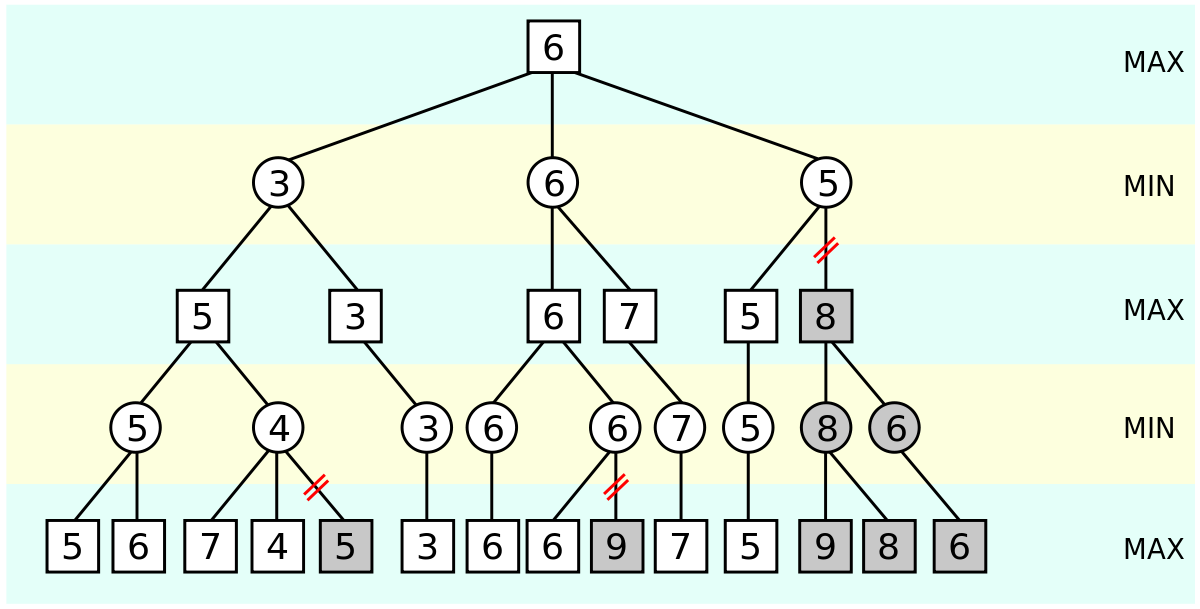
\includegraphics[width=.90\textwidth]{pruning.svg.png}
	\caption{Überblick über die Vorgehensweise des Alpha-Beta-Prunings\footnotemark}
	\label{fig:pruning}
\end{figure}
\footnotetext{\cite{pruning}}

Genauer erklärt, werden für diese Erweiterung des Algorithmus zwei weitere Werte verwendet: $Alpha$ und $Beta$. Diese beiden Werte stellen zwei Grenzen dar, welche als Worst-Case-Szenarios gesehen werden können. Der Wert $Alpha$ stellt die untere Grenze und somit das Worst-Case-Szenario für die KI dar, während $Beta$ die obere Grenze und somit das Worst-Case-Szenario für den menschlichen Spieler abbildet. Der Algorithmus läuft so ab, dass mithilfe der Schranken die Werte der Zustands-Evaluation überprüft werden; überschreitet ein Wert die $Beta$-Grenze, so wird der gesamte Teilbaum von diesem Knoten ausgehend "`abgeschnitten"' -- ergo nicht weiter betrachtet -- da die gegnerische Seite (der menschliche Spieler) diesen Teilbaum nicht betreten wird, weil die bisher evaluierten Teilbäume bereits bessere Ergebnisse für den Spielern liefern. Die $Alpha$-Grenze wird so verwendet, dass die Werte der Zustands-Evaluation nur dann übernommen -- und somit als neuer $Alpha$-Wert gesetzt werden -- werden, falls sie die die bestehende $Alpha$-Grenze nicht unterschreiten, da in diesem Fall der betrachtete Zug schlechter als der aktuell beste Zug wäre.

\section{Implementierung}
In diesem Abschnitt wird demonstriert, wie der oben erwähnte Algorithmus praktisch umgesetzt wurde. Es wird nicht der vollständige Code gezeigt, sondern lediglich die Haupt-Funktion des Minimax-Algorithmus, da sich diese Arbeit weniger auf den bereits vorhandenen Algorithmus fokussiert, sondern mehr auf die Implementierung der Quiescence Search. In Kapitel~\ref{ch:quiescence} hingegen wird der gesamte Code gezeigt, der im Rahmen der Implementierung geschrieben wurde. Es sei an dieser Stelle nichtsdestotrotz erneut auf \url{https://github.com/felixwortmann/chess} verwiesen, wo der gesamte Quellcode für die Schach-KI sowie diverse Hilfs- und Testfunktionen abrufbar ist.

\begin{lstlisting}[caption=Funktion für den Minimax-Algorithmus mit Alpha-Beta-Pruning, label=lst:algo]
@memoize_minimax
def minimax(board, depth, alpha, beta):
    global BEST_MOVE
    global MINIMAX_CALLS
    MINIMAX_CALLS += 1
    # Check, if current board is in cache
    # If the depth is zero, give the static evaluation of the current board and save it in the cache
    if depth == 0 or not board.legal_moves:
        value = static_eval(board, is_endgame(board))
        return value
    max_value = alpha
    ordered_moves = []
    cnt = 0
    # Order the moves roughly, using a static evaluation for every move
    for move in board.legal_moves:
        cnt += 1
        board.push(move)
        v = static_eval(board, is_endgame(board))
        board.pop()
        heapq.heappush(ordered_moves, (v, cnt, move))
    # Calculate the minimax value recursively, using alpha-beta-pruning
    for _, _, move in ordered_moves:
        board.push(move)
        value = -minimax(board, depth - 1, -beta, -max_value)
        board.pop()
        if value > max_value:
            max_value = value
            if depth == ANALYZING_DEPTH:
                BEST_MOVE = move
            if max_value >= beta:
                break
    return max_value
\end{lstlisting}

Das Code-Beispiel~\ref{lst:algo} zeigt die Funktion, welche den Minimax-Algorithmus implementiert. Es sei erneut erwähnt, dass es sich technisch gesehen um einen Negamax-Algorithmus handelt, weshalb in der Funktion keine Unterscheidung zwischen maximierendem und minimierendem Spieler gemacht wird. Stattdessen werden die Werte bei Aufruf der Funktion sowie der zurückgegebene Wert des rekursiven Aufrufs invertiert.

Die Funktion wird mit den folgenden Parametern aufgerufen:

\begin{itemize}
    \item \texttt{board}, der Zustand des aktuellen Spielbrettes. Für das Brett wurde die Python-Bibliothek \textit{python-chess} verwendet
    \item \texttt{depth}, zu Beginn die gewünschte Suchtiefe (standardmäßig beträgt diese $5$), danach verringert sich der Wert mit jedem rekursiven Aufruf
    \item \texttt{alpha} und \texttt{beta}, die oben erwähnten Werte, welche die Schranken für das Alpha-Beta-Pruning darstellen
\end{itemize}

Der Ablauf der Funktion lässt sich folgendermaßen zusammenfassen:

\begin{enumerate}
    \item Zunächst wird geprüft, ob die Tiefe $0$ beträgt, die Funktion also "`unten"' am Baum angekommen ist, oder keine weiteren Züge zur Analyse vorhanden sind. In diesem Fall wird die Auswertung der aktuellen Spielposition zurückgegeben
    \item Anschließend, falls Punkt 1 übersprungen wurde, werden die vorhandenen Züge grob sortiert, indem auf sie die Evaluations-Funktion angewendet wird und sie anschließend anhand dessen sortiert werden
    \item Nun wird durch die sortierten Züge iteriert und die Funktion ruft sich rekursiv selbst auf. Der Rückgabewert wird invertiert (aufgrund der Negamax-Variante) und das Alpha-Beta-Pruning wird angewendet
\end{enumerate}

Die Sortierung der Züge verbessert die Performanz der Schach-KI zusätzlich, da das Alpha-Beta-Pruning so deutlich effektiver angewendet werden kann.